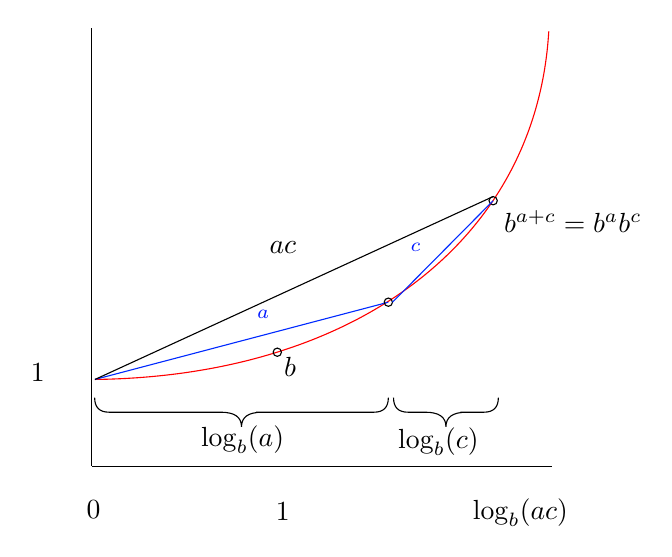
\begin{tikzpicture}[x=0.75pt,y=0.75pt,yscale=-1,xscale=1]
%uncomment if require: \path (0,300); %set diagram left start at 0, and has height of 300

%Curve Lines [id:da03288993175087518] 
\draw [color={rgb, 255:red, 255; green, 0; blue, 0 }  ,draw opacity=1 ]   (155.15,179.22) .. controls (279.44,177.72) and (367.8,113.33) .. (373.79,11.5) ;
%Straight Lines [id:da1130487867315304] 
\draw    (153.65,221.15) -- (375.28,221.15) ;
%Straight Lines [id:da33259651715487903] 
\draw    (153.65,10) -- (153.65,221.15) ;
%Shape: Circle [id:dp08048097645129337] 
\draw   (345,93.1) .. controls (345,91.99) and (345.9,91.1) .. (347,91.1) .. controls (348.1,91.1) and (349,91.99) .. (349,93.1) .. controls (349,94.2) and (348.1,95.1) .. (347,95.1) .. controls (345.9,95.1) and (345,94.2) .. (345,93.1) -- cycle ;
%Shape: Circle [id:dp0349937774727469] 
\draw   (241,166.1) .. controls (241,164.99) and (241.9,164.1) .. (243,164.1) .. controls (244.1,164.1) and (245,164.99) .. (245,166.1) .. controls (245,167.2) and (244.1,168.1) .. (243,168.1) .. controls (241.9,168.1) and (241,167.2) .. (241,166.1) -- cycle ;
%Straight Lines [id:da4023477966991159] 
\draw [color={rgb, 255:red, 0; green, 42; blue, 255 }  ,draw opacity=1 ]   (155.15,179.22) -- (296.5,142) ;
%Shape: Circle [id:dp6857242879889043] 
\draw   (294.5,142) .. controls (294.5,140.9) and (295.4,140) .. (296.5,140) .. controls (297.6,140) and (298.5,140.9) .. (298.5,142) .. controls (298.5,143.1) and (297.6,144) .. (296.5,144) .. controls (295.4,144) and (294.5,143.1) .. (294.5,142) -- cycle ;
%Straight Lines [id:da4161013432719185] 
\draw [color={rgb, 255:red, 0; green, 42; blue, 255 }  ,draw opacity=1 ]   (298.5,142) -- (347,93.1) ;
%Straight Lines [id:da5038115107934119] 
\draw    (155.15,179.22) -- (347,91.1) ;
%Shape: Brace [id:dp5633640978469883] 
\draw   (155,188) .. controls (155,192.67) and (157.33,195) .. (162,195) -- (215.75,195) .. controls (222.42,195) and (225.75,197.33) .. (225.75,202) .. controls (225.75,197.33) and (229.08,195) .. (235.75,195)(232.75,195) -- (289.5,195) .. controls (294.17,195) and (296.5,192.67) .. (296.5,188) ;
%Shape: Brace [id:dp3308211831927511] 
\draw   (299,188) .. controls (299,192.67) and (301.33,195) .. (306,195) -- (314.25,195) .. controls (320.92,195) and (324.25,197.33) .. (324.25,202) .. controls (324.25,197.33) and (327.58,195) .. (334.25,195)(331.25,195) -- (342.5,195) .. controls (347.17,195) and (349.5,192.67) .. (349.5,188) ;

% Text Node
\draw (149.9,236.5) node [anchor=north west][inner sep=0.75pt]    {$0$};
% Text Node
\draw (123,170.5) node [anchor=north west][inner sep=0.75pt]    {$1$};
% Text Node
\draw (351,96.5) node [anchor=north west][inner sep=0.75pt]    {$b^{a+c} =b^{a} b^{c}$};
% Text Node
\draw (245,167.5) node [anchor=north west][inner sep=0.75pt]    {$b$};
% Text Node
\draw (241,237.5) node [anchor=north west][inner sep=0.75pt]    {$1$};
% Text Node
\draw (336,235.5) node [anchor=north west][inner sep=0.75pt]    {$\log_{b}( ac)$};
% Text Node
\draw (232,144.4) node [anchor=north west][inner sep=0.75pt]  [font=\scriptsize,color={rgb, 255:red, 0; green, 24; blue, 255 }  ,opacity=1 ]  {$a$};
% Text Node
\draw (306,112.4) node [anchor=north west][inner sep=0.75pt]  [font=\scriptsize,color={rgb, 255:red, 0; green, 24; blue, 255 }  ,opacity=1 ]  {$c$};
% Text Node
\draw (238,111.4) node [anchor=north west][inner sep=0.75pt]    {$ac$};
% Text Node
\draw (205,200.4) node [anchor=north west][inner sep=0.75pt]    {$\log_{b}( a)$};
% Text Node
\draw (300,201.4) node [anchor=north west][inner sep=0.75pt]    {$\log_{b}( c)$};


\end{tikzpicture}